% Options for packages loaded elsewhere
\PassOptionsToPackage{unicode}{hyperref}
\PassOptionsToPackage{hyphens}{url}
\PassOptionsToPackage{dvipsnames,svgnames,x11names}{xcolor}
%
\documentclass[
  letterpaper,
  DIV=11,
  numbers=noendperiod]{scrartcl}

\usepackage{amsmath,amssymb}
\usepackage{iftex}
\ifPDFTeX
  \usepackage[T1]{fontenc}
  \usepackage[utf8]{inputenc}
  \usepackage{textcomp} % provide euro and other symbols
\else % if luatex or xetex
  \usepackage{unicode-math}
  \defaultfontfeatures{Scale=MatchLowercase}
  \defaultfontfeatures[\rmfamily]{Ligatures=TeX,Scale=1}
\fi
\usepackage{lmodern}
\ifPDFTeX\else  
    % xetex/luatex font selection
\fi
% Use upquote if available, for straight quotes in verbatim environments
\IfFileExists{upquote.sty}{\usepackage{upquote}}{}
\IfFileExists{microtype.sty}{% use microtype if available
  \usepackage[]{microtype}
  \UseMicrotypeSet[protrusion]{basicmath} % disable protrusion for tt fonts
}{}
\makeatletter
\@ifundefined{KOMAClassName}{% if non-KOMA class
  \IfFileExists{parskip.sty}{%
    \usepackage{parskip}
  }{% else
    \setlength{\parindent}{0pt}
    \setlength{\parskip}{6pt plus 2pt minus 1pt}}
}{% if KOMA class
  \KOMAoptions{parskip=half}}
\makeatother
\usepackage{xcolor}
\setlength{\emergencystretch}{3em} % prevent overfull lines
\setcounter{secnumdepth}{-\maxdimen} % remove section numbering
% Make \paragraph and \subparagraph free-standing
\makeatletter
\ifx\paragraph\undefined\else
  \let\oldparagraph\paragraph
  \renewcommand{\paragraph}{
    \@ifstar
      \xxxParagraphStar
      \xxxParagraphNoStar
  }
  \newcommand{\xxxParagraphStar}[1]{\oldparagraph*{#1}\mbox{}}
  \newcommand{\xxxParagraphNoStar}[1]{\oldparagraph{#1}\mbox{}}
\fi
\ifx\subparagraph\undefined\else
  \let\oldsubparagraph\subparagraph
  \renewcommand{\subparagraph}{
    \@ifstar
      \xxxSubParagraphStar
      \xxxSubParagraphNoStar
  }
  \newcommand{\xxxSubParagraphStar}[1]{\oldsubparagraph*{#1}\mbox{}}
  \newcommand{\xxxSubParagraphNoStar}[1]{\oldsubparagraph{#1}\mbox{}}
\fi
\makeatother

\usepackage{color}
\usepackage{fancyvrb}
\newcommand{\VerbBar}{|}
\newcommand{\VERB}{\Verb[commandchars=\\\{\}]}
\DefineVerbatimEnvironment{Highlighting}{Verbatim}{commandchars=\\\{\}}
% Add ',fontsize=\small' for more characters per line
\usepackage{framed}
\definecolor{shadecolor}{RGB}{241,243,245}
\newenvironment{Shaded}{\begin{snugshade}}{\end{snugshade}}
\newcommand{\AlertTok}[1]{\textcolor[rgb]{0.68,0.00,0.00}{#1}}
\newcommand{\AnnotationTok}[1]{\textcolor[rgb]{0.37,0.37,0.37}{#1}}
\newcommand{\AttributeTok}[1]{\textcolor[rgb]{0.40,0.45,0.13}{#1}}
\newcommand{\BaseNTok}[1]{\textcolor[rgb]{0.68,0.00,0.00}{#1}}
\newcommand{\BuiltInTok}[1]{\textcolor[rgb]{0.00,0.23,0.31}{#1}}
\newcommand{\CharTok}[1]{\textcolor[rgb]{0.13,0.47,0.30}{#1}}
\newcommand{\CommentTok}[1]{\textcolor[rgb]{0.37,0.37,0.37}{#1}}
\newcommand{\CommentVarTok}[1]{\textcolor[rgb]{0.37,0.37,0.37}{\textit{#1}}}
\newcommand{\ConstantTok}[1]{\textcolor[rgb]{0.56,0.35,0.01}{#1}}
\newcommand{\ControlFlowTok}[1]{\textcolor[rgb]{0.00,0.23,0.31}{\textbf{#1}}}
\newcommand{\DataTypeTok}[1]{\textcolor[rgb]{0.68,0.00,0.00}{#1}}
\newcommand{\DecValTok}[1]{\textcolor[rgb]{0.68,0.00,0.00}{#1}}
\newcommand{\DocumentationTok}[1]{\textcolor[rgb]{0.37,0.37,0.37}{\textit{#1}}}
\newcommand{\ErrorTok}[1]{\textcolor[rgb]{0.68,0.00,0.00}{#1}}
\newcommand{\ExtensionTok}[1]{\textcolor[rgb]{0.00,0.23,0.31}{#1}}
\newcommand{\FloatTok}[1]{\textcolor[rgb]{0.68,0.00,0.00}{#1}}
\newcommand{\FunctionTok}[1]{\textcolor[rgb]{0.28,0.35,0.67}{#1}}
\newcommand{\ImportTok}[1]{\textcolor[rgb]{0.00,0.46,0.62}{#1}}
\newcommand{\InformationTok}[1]{\textcolor[rgb]{0.37,0.37,0.37}{#1}}
\newcommand{\KeywordTok}[1]{\textcolor[rgb]{0.00,0.23,0.31}{\textbf{#1}}}
\newcommand{\NormalTok}[1]{\textcolor[rgb]{0.00,0.23,0.31}{#1}}
\newcommand{\OperatorTok}[1]{\textcolor[rgb]{0.37,0.37,0.37}{#1}}
\newcommand{\OtherTok}[1]{\textcolor[rgb]{0.00,0.23,0.31}{#1}}
\newcommand{\PreprocessorTok}[1]{\textcolor[rgb]{0.68,0.00,0.00}{#1}}
\newcommand{\RegionMarkerTok}[1]{\textcolor[rgb]{0.00,0.23,0.31}{#1}}
\newcommand{\SpecialCharTok}[1]{\textcolor[rgb]{0.37,0.37,0.37}{#1}}
\newcommand{\SpecialStringTok}[1]{\textcolor[rgb]{0.13,0.47,0.30}{#1}}
\newcommand{\StringTok}[1]{\textcolor[rgb]{0.13,0.47,0.30}{#1}}
\newcommand{\VariableTok}[1]{\textcolor[rgb]{0.07,0.07,0.07}{#1}}
\newcommand{\VerbatimStringTok}[1]{\textcolor[rgb]{0.13,0.47,0.30}{#1}}
\newcommand{\WarningTok}[1]{\textcolor[rgb]{0.37,0.37,0.37}{\textit{#1}}}

\providecommand{\tightlist}{%
  \setlength{\itemsep}{0pt}\setlength{\parskip}{0pt}}\usepackage{longtable,booktabs,array}
\usepackage{calc} % for calculating minipage widths
% Correct order of tables after \paragraph or \subparagraph
\usepackage{etoolbox}
\makeatletter
\patchcmd\longtable{\par}{\if@noskipsec\mbox{}\fi\par}{}{}
\makeatother
% Allow footnotes in longtable head/foot
\IfFileExists{footnotehyper.sty}{\usepackage{footnotehyper}}{\usepackage{footnote}}
\makesavenoteenv{longtable}
\usepackage{graphicx}
\makeatletter
\def\maxwidth{\ifdim\Gin@nat@width>\linewidth\linewidth\else\Gin@nat@width\fi}
\def\maxheight{\ifdim\Gin@nat@height>\textheight\textheight\else\Gin@nat@height\fi}
\makeatother
% Scale images if necessary, so that they will not overflow the page
% margins by default, and it is still possible to overwrite the defaults
% using explicit options in \includegraphics[width, height, ...]{}
\setkeys{Gin}{width=\maxwidth,height=\maxheight,keepaspectratio}
% Set default figure placement to htbp
\makeatletter
\def\fps@figure{htbp}
\makeatother

\KOMAoption{captions}{tableheading}
\makeatletter
\@ifpackageloaded{caption}{}{\usepackage{caption}}
\AtBeginDocument{%
\ifdefined\contentsname
  \renewcommand*\contentsname{Table of contents}
\else
  \newcommand\contentsname{Table of contents}
\fi
\ifdefined\listfigurename
  \renewcommand*\listfigurename{List of Figures}
\else
  \newcommand\listfigurename{List of Figures}
\fi
\ifdefined\listtablename
  \renewcommand*\listtablename{List of Tables}
\else
  \newcommand\listtablename{List of Tables}
\fi
\ifdefined\figurename
  \renewcommand*\figurename{Figure}
\else
  \newcommand\figurename{Figure}
\fi
\ifdefined\tablename
  \renewcommand*\tablename{Table}
\else
  \newcommand\tablename{Table}
\fi
}
\@ifpackageloaded{float}{}{\usepackage{float}}
\floatstyle{ruled}
\@ifundefined{c@chapter}{\newfloat{codelisting}{h}{lop}}{\newfloat{codelisting}{h}{lop}[chapter]}
\floatname{codelisting}{Listing}
\newcommand*\listoflistings{\listof{codelisting}{List of Listings}}
\makeatother
\makeatletter
\makeatother
\makeatletter
\@ifpackageloaded{caption}{}{\usepackage{caption}}
\@ifpackageloaded{subcaption}{}{\usepackage{subcaption}}
\makeatother

\ifLuaTeX
  \usepackage{selnolig}  % disable illegal ligatures
\fi
\usepackage{bookmark}

\IfFileExists{xurl.sty}{\usepackage{xurl}}{} % add URL line breaks if available
\urlstyle{same} % disable monospaced font for URLs
\hypersetup{
  pdftitle={CHL8010: Statistical Programming and Computation in Health Data},
  pdfauthor={Week 4 In-class Assignment},
  colorlinks=true,
  linkcolor={blue},
  filecolor={Maroon},
  citecolor={Blue},
  urlcolor={Blue},
  pdfcreator={LaTeX via pandoc}}


\title{CHL8010: Statistical Programming and Computation in Health Data}
\author{Week 4 In-class Assignment}
\date{2024-09-30}

\begin{document}
\maketitle


\begin{Shaded}
\begin{Highlighting}[]
\FunctionTok{library}\NormalTok{(here)}
\end{Highlighting}
\end{Shaded}

\begin{verbatim}
here() starts at C:/Users/temoo/OneDrive/Desktop/Uni/Year MPH 1/Year 2/Stat computation/ArmedConflict
\end{verbatim}

\begin{Shaded}
\begin{Highlighting}[]
\FunctionTok{library}\NormalTok{(ggcorrplot)}
\end{Highlighting}
\end{Shaded}

\begin{verbatim}
Loading required package: ggplot2
\end{verbatim}

\begin{Shaded}
\begin{Highlighting}[]
\FunctionTok{library}\NormalTok{(ggplot2)}
\FunctionTok{library}\NormalTok{(dplyr)}
\end{Highlighting}
\end{Shaded}

\begin{verbatim}

Attaching package: 'dplyr'
\end{verbatim}

\begin{verbatim}
The following objects are masked from 'package:stats':

    filter, lag
\end{verbatim}

\begin{verbatim}
The following objects are masked from 'package:base':

    intersect, setdiff, setequal, union
\end{verbatim}

\begin{Shaded}
\begin{Highlighting}[]
\FunctionTok{source}\NormalTok{(}\FunctionTok{here}\NormalTok{(}\StringTok{"R"}\NormalTok{, }\StringTok{"merged\_dataset.R"}\NormalTok{))}
\end{Highlighting}
\end{Shaded}

\begin{verbatim}
[1] "Columns with NA values:"
     gdp1000      popdens        urban     male_edu         temp rainfall1000 
          62           20           20           20           20           20 
      MarMor      InfMort NeonatalMort   Under5Mort      Drought   Earthquake 
         426           20           20           20         3132         3132 
# A tibble: 0 x 2
# i 2 variables: ISO <chr>, count <int>
\end{verbatim}

\subsection{Perfect your GitHub repo}\label{perfect-your-github-repo}

Some of you may still need to organize your GitHub repo. Use this time
to do that. When you are confident with your repo, let me know -- I will
try to reproduce your code.

Your final data should have the following variables (you might have
slightly different variable names).

\begin{Shaded}
\begin{Highlighting}[]
\NormalTok{finaldata }\OtherTok{\textless{}{-}} \FunctionTok{read.csv}\NormalTok{(}\FunctionTok{here}\NormalTok{(}\StringTok{"data"}\NormalTok{, }\StringTok{"analytical"}\NormalTok{, }\StringTok{"finaldata.csv"}\NormalTok{), }\AttributeTok{header =} \ConstantTok{TRUE}\NormalTok{)}
\FunctionTok{names}\NormalTok{(finaldata)}
\end{Highlighting}
\end{Shaded}

\begin{verbatim}
 [1] "country_name" "ISO"          "region"       "Year"         "gdp1000"     
 [6] "OECD"         "OECD2023"     "popdens"      "urban"        "agedep"      
[11] "male_edu"     "temp"         "rainfall1000" "MarMor"       "InfMort"     
[16] "NeonatalMort" "Under5Mort"   "total_deaths" "conflict"     "Drought"     
[21] "Earthquake"  
\end{verbatim}

Observations from Canada should look like this\ldots{}

\begin{Shaded}
\begin{Highlighting}[]
\NormalTok{finaldata }\SpecialCharTok{\%\textgreater{}\%}
\NormalTok{  dplyr}\SpecialCharTok{::}\FunctionTok{filter}\NormalTok{(country\_name }\SpecialCharTok{==} \StringTok{"Canada"}\NormalTok{)}
\end{Highlighting}
\end{Shaded}

\begin{verbatim}
   country_name ISO           region Year  gdp1000 OECD OECD2023  popdens
1        Canada CAN Northern America 2000 24.27100    1        1 66.19704
2        Canada CAN Northern America 2001 23.82206    1        1 66.45361
3        Canada CAN Northern America 2002 24.25534    1        1 66.71112
4        Canada CAN Northern America 2003 28.30046    1        1 66.96384
5        Canada CAN Northern America 2004 32.14368    1        1 67.21715
6        Canada CAN Northern America 2005 36.38251    1        1 67.47283
7        Canada CAN Northern America 2006 40.50406    1        1 67.73674
8        Canada CAN Northern America 2007 44.65990    1        1 67.99444
9        Canada CAN Northern America 2008 46.71051    1        1 68.25765
10       Canada CAN Northern America 2009 40.87631    1        1 68.53354
11       Canada CAN Northern America 2010 47.56208    1        1 68.80739
12       Canada CAN Northern America 2011 52.22370    1        1 69.04842
13       Canada CAN Northern America 2012 52.66909    1        1 69.27604
14       Canada CAN Northern America 2013 52.63517    1        1 69.50772
15       Canada CAN Northern America 2014 50.95600    1        1 69.76876
16       Canada CAN Northern America 2015 43.59614    1        1 69.98853
17       Canada CAN Northern America 2016 42.31560    1        1 70.21484
18       Canada CAN Northern America 2017 45.12943    1        1 70.40863
19       Canada CAN Northern America 2018 46.54864    1        1 70.63614
20       Canada CAN Northern America 2019 46.32867    1        1 70.83794
      urban   agedep male_edu     temp rainfall1000 MarMor InfMort NeonatalMort
1  56.14335 46.34463 12.30281 5.486244    0.9971559      9     5.3          3.8
2  56.40270 45.89632 12.35258 6.469105    0.8644873     10     5.3          3.8
3  56.67093 45.46660 12.40182 5.979147    0.9460938     10     5.3          3.9
4  56.94365 45.07468 12.45053 5.416964    1.0189234     10     5.3          3.9
5  57.20020 44.67374 12.49870 5.556961    1.0008237     10     5.3          3.9
6  57.41671 44.26641 12.54635 6.187472    1.0367199     11     5.2          3.9
7  57.59143 43.96370 12.59349 6.895084    1.0917386     11     5.2          3.9
8  57.75691 43.83612 12.64015 5.900051    1.0134091     11     5.1          3.8
9  57.97905 43.85426 12.68634 5.650118    1.0693435     12     5.1          3.8
10 58.24228 43.94937 12.73207 5.398867    0.9928497     12     5.0          3.8
11 58.52809 44.13587 12.77735 6.781766    1.0379754     11     5.0          3.8
12 58.81437 44.53578 12.82218 6.269133    1.1343442     11     4.9          3.7
13 59.05573 45.18393 12.86660 7.249497    0.9747708     11     4.9          3.7
14 59.19713 45.95404 12.91059 5.954381    1.0282075     11     4.8          3.6
15 59.30361 46.75493 12.95414 5.584650    1.0377695     11     4.7          3.6
16 59.42627 47.59164 12.99723 6.436884    0.9632446     11     4.7          3.6
17 59.50521 48.41410 13.03988 7.184514    0.9677826     10     4.6          3.5
18 59.59325 49.14806 13.08210 6.539669    1.0995322     10     4.6          3.4
19 59.68433 49.80166 13.12388 6.539677    1.0991469     NA     4.5          3.3
20 59.75984 50.47739 13.16522 6.539633    1.0987523     NA     4.4          3.3
   Under5Mort total_deaths conflict Drought Earthquake
1         6.2           11        0       0          0
2         6.2           23        0       0          0
3         6.2            1        0       0          0
4         6.2            0        0       0          0
5         6.1            0        0       0          0
6         6.1            0        0       0          0
7         6.0            0        0       0          0
8         6.0            0        0       0          0
9         5.9            0        0       0          0
10        5.8            0        0       0          0
11        5.7            0        0       0          0
12        5.7            0        0       0          0
13        5.6            0        0       0          0
14        5.5            0        0       0          0
15        5.4            0        0       0          0
16        5.4            0        0       0          0
17        5.3            0        0       0          0
18        5.2            0        0       0          0
19        5.1            0        0       0          0
20        5.1            0        0       0          0
\end{verbatim}

Observations from Ecuador should look like this\ldots{}

\begin{Shaded}
\begin{Highlighting}[]
\NormalTok{finaldata }\SpecialCharTok{\%\textgreater{}\%}
\NormalTok{  dplyr}\SpecialCharTok{::}\FunctionTok{filter}\NormalTok{(country\_name }\SpecialCharTok{==} \StringTok{"Ecuador"}\NormalTok{)}
\end{Highlighting}
\end{Shaded}

\begin{verbatim}
   country_name ISO                          region Year  gdp1000 OECD OECD2023
1       Ecuador ECU Latin America and the Caribbean 2000 1.451531    0        0
2       Ecuador ECU Latin America and the Caribbean 2001 1.904814    0        0
3       Ecuador ECU Latin America and the Caribbean 2002 2.184209    0        0
4       Ecuador ECU Latin America and the Caribbean 2003 2.438344    0        0
5       Ecuador ECU Latin America and the Caribbean 2004 2.703566    0        0
6       Ecuador ECU Latin America and the Caribbean 2005 3.014310    0        0
7       Ecuador ECU Latin America and the Caribbean 2006 3.340841    0        0
8       Ecuador ECU Latin America and the Caribbean 2007 3.579032    0        0
9       Ecuador ECU Latin America and the Caribbean 2008 4.260433    0        0
10      Ecuador ECU Latin America and the Caribbean 2009 4.240703    0        0
11      Ecuador ECU Latin America and the Caribbean 2010 4.640246    0        0
12      Ecuador ECU Latin America and the Caribbean 2011 5.202656    0        0
13      Ecuador ECU Latin America and the Caribbean 2012 5.678456    0        0
14      Ecuador ECU Latin America and the Caribbean 2013 6.050355    0        0
15      Ecuador ECU Latin America and the Caribbean 2014 6.374631    0        0
16      Ecuador ECU Latin America and the Caribbean 2015 6.130587    0        0
17      Ecuador ECU Latin America and the Caribbean 2016 6.079089    0        0
18      Ecuador ECU Latin America and the Caribbean 2017 6.246404    0        0
19      Ecuador ECU Latin America and the Caribbean 2018 6.321349    0        0
20      Ecuador ECU Latin America and the Caribbean 2019 6.233258    0        0
    popdens    urban   agedep male_edu     temp rainfall1000 MarMor InfMort
1  23.27432 36.19963 67.44216 7.738627 19.54855    1.4201653    122    24.7
2  23.39372 36.67994 66.57356 7.843942 19.66622    1.1667746    117    23.4
3  23.52087 37.08903 65.65488 7.949449 20.24695    1.4577981    110    22.4
4  23.58358 37.23792 64.71472 8.055240 20.05016    1.5781807    100    21.5
5  38.43743 37.39268 63.78049 8.161433 20.10136    1.0683450     94    20.7
6  38.55361 37.36968 62.86530 8.268176 19.88163    0.8555447     94    19.9
7  38.65018 37.47567 61.97042 8.375587 20.07087    1.1114502     90    19.2
8  38.76505 37.68172 61.11422 8.483729 19.49536    1.0899082     85    18.5
9  38.83977 37.67445 60.31015 8.592603 19.85711    1.6184816     82    17.7
10 38.92613 37.39437 59.55262 8.702180 20.39298    1.0870796     80    17.0
11 39.03066 37.26838 58.83793 8.812409 20.11160    1.7045703     78    16.3
12 39.09586 37.61553 58.16553 8.923172 19.86633    1.4518388     76    15.6
13 39.13343 38.00733 57.51051 9.034284 20.19000    1.7520003     71    14.9
14 39.18619 38.22511 56.84804 9.145523 19.85177    1.3735605     67    14.3
15 39.27871 38.12421 56.17001 9.256679 20.42252    1.2572257     65    13.7
16 39.38824 38.15633 55.46511 9.367582 20.95595    1.7284273     63    13.2
17 39.46201 38.45745 54.73369 9.478071 20.77476    1.3168761     61    12.8
18 39.53609 38.65993 53.99096 9.587993 20.53262    1.9544485     59    12.4
19 39.58380 38.87253 53.12249 9.697221 20.53714    1.9573265     NA    12.0
20 39.75109 39.05144 52.29278 9.805670 20.54169    1.9602443     NA    11.6
   NeonatalMort Under5Mort total_deaths conflict Drought Earthquake
1          14.1       29.5            0        0       0          0
2          13.4       28.0            0        0       0          0
3          12.7       26.6            2        0       0          0
4          12.1       25.4            0        0       0          0
5          11.6       24.4           26        1       0          0
6          11.1       23.5            0        0       0          0
7          10.6       22.6            0        0       0          0
8          10.2       21.7            0        0       0          0
9           9.7       20.8            0        0       0          0
10          9.3       19.9           25        1       1          0
11          8.9       19.0            0        0       0          0
12          8.5       18.1            0        0       0          0
13          8.1       17.3            0        0       0          0
14          7.8       16.6            0        0       1          0
15          7.5       15.9            0        0       0          1
16          7.3       15.4            0        0       0          0
17          7.1       14.8            0        0       0          1
18          6.9       14.4            0        0       0          0
19          6.9       13.9            0        0       0          0
20          6.8       13.4            0        0       0          1
\end{verbatim}

\subsection{Exploratory data analysis}\label{exploratory-data-analysis}

Use the rest of the class time to explore the final data that will be
used for analysis starting next week. At the end of the class, write a
summary of your findings and push your \textbf{Quarto document (pdf)} to
your repo.

\begin{Shaded}
\begin{Highlighting}[]
\FunctionTok{summary}\NormalTok{(finaldata)}
\end{Highlighting}
\end{Shaded}

\begin{verbatim}
 country_name           ISO               region               Year     
 Length:3720        Length:3720        Length:3720        Min.   :2000  
 Class :character   Class :character   Class :character   1st Qu.:2005  
 Mode  :character   Mode  :character   Mode  :character   Median :2010  
                                                          Mean   :2010  
                                                          3rd Qu.:2014  
                                                          Max.   :2019  
                                                                        
    gdp1000              OECD          OECD2023         popdens     
 Min.   :  0.1105   Min.   :0.000   Min.   :0.0000   Min.   : 0.00  
 1st Qu.:  1.2383   1st Qu.:0.000   1st Qu.:0.0000   1st Qu.:14.79  
 Median :  4.0719   Median :0.000   Median :0.0000   Median :27.52  
 Mean   : 11.4917   Mean   :0.171   Mean   :0.1882   Mean   :30.57  
 3rd Qu.: 13.1531   3rd Qu.:0.000   3rd Qu.:0.0000   3rd Qu.:40.72  
 Max.   :123.6787   Max.   :1.000   Max.   :1.0000   Max.   :99.86  
 NA's   :62                                          NA's   :20     
     urban             agedep          male_edu           temp       
 Min.   : 0.1025   Min.   : 16.17   Min.   : 1.067   Min.   :-2.405  
 1st Qu.:17.2872   1st Qu.: 47.94   1st Qu.: 5.904   1st Qu.:12.928  
 Median :30.2535   Median : 55.51   Median : 8.368   Median :21.958  
 Mean   :30.6948   Mean   : 61.94   Mean   : 8.258   Mean   :19.625  
 3rd Qu.:41.6558   3rd Qu.: 77.11   3rd Qu.:10.849   3rd Qu.:25.869  
 Max.   :93.4135   Max.   :111.48   Max.   :14.441   Max.   :29.676  
 NA's   :20                         NA's   :20       NA's   :20      
  rainfall1000         MarMor          InfMort        NeonatalMort  
 Min.   :0.01993   Min.   :   2.0   Min.   :  1.60   Min.   : 0.80  
 1st Qu.:0.59146   1st Qu.:  17.0   1st Qu.:  7.60   1st Qu.: 4.90  
 Median :1.01288   Median :  66.0   Median : 18.90   Median :12.10  
 Mean   :1.20216   Mean   : 210.6   Mean   : 28.90   Mean   :16.18  
 3rd Qu.:1.68706   3rd Qu.: 299.8   3rd Qu.: 44.52   3rd Qu.:25.32  
 Max.   :4.71081   Max.   :2480.0   Max.   :138.10   Max.   :60.90  
 NA's   :20        NA's   :426      NA's   :20       NA's   :20     
   Under5Mort      total_deaths        conflict         Drought       
 Min.   :  2.00   Min.   :    0.0   Min.   :0.0000   Min.   :0.00000  
 1st Qu.:  9.00   1st Qu.:    0.0   1st Qu.:0.0000   1st Qu.:0.00000  
 Median : 22.20   Median :    0.0   Median :0.0000   Median :0.00000  
 Mean   : 40.50   Mean   :  361.1   Mean   :0.1892   Mean   :0.08737  
 3rd Qu.: 61.33   3rd Qu.:    2.0   3rd Qu.:0.0000   3rd Qu.:0.00000  
 Max.   :224.90   Max.   :78644.0   Max.   :1.0000   Max.   :1.00000  
 NA's   :20                                                           
   Earthquake     
 Min.   :0.00000  
 1st Qu.:0.00000  
 Median :0.00000  
 Mean   :0.08333  
 3rd Qu.:0.00000  
 Max.   :1.00000  
                  
\end{verbatim}

\begin{Shaded}
\begin{Highlighting}[]
\CommentTok{\# Check for missing values}
\FunctionTok{colSums}\NormalTok{(}\FunctionTok{is.na}\NormalTok{(finaldata))}
\end{Highlighting}
\end{Shaded}

\begin{verbatim}
country_name          ISO       region         Year      gdp1000         OECD 
           0            0            0            0           62            0 
    OECD2023      popdens        urban       agedep     male_edu         temp 
           0           20           20            0           20           20 
rainfall1000       MarMor      InfMort NeonatalMort   Under5Mort total_deaths 
          20          426           20           20           20            0 
    conflict      Drought   Earthquake 
           0            0            0 
\end{verbatim}

gdp1000, popdens, urban, male\_edu, temp, rainfall1000, MarMor, InfMort,
NeonatalMort all have missing data

MarMor has a lot of missing data

\begin{Shaded}
\begin{Highlighting}[]
\CommentTok{\#Bivariate analysis}

\CommentTok{\#GDP and Population density}
\FunctionTok{ggplot}\NormalTok{(finaldata, }\FunctionTok{aes}\NormalTok{(}\AttributeTok{x=}\NormalTok{gdp1000, }\AttributeTok{y=}\NormalTok{popdens)) }\SpecialCharTok{+} 
  \FunctionTok{geom\_point}\NormalTok{() }\SpecialCharTok{+} 
  \FunctionTok{labs}\NormalTok{(}\AttributeTok{title=}\StringTok{"GDP vs Population Density"}\NormalTok{)}
\end{Highlighting}
\end{Shaded}

\begin{verbatim}
Warning: Removed 82 rows containing missing values or values outside the scale range
(`geom_point()`).
\end{verbatim}

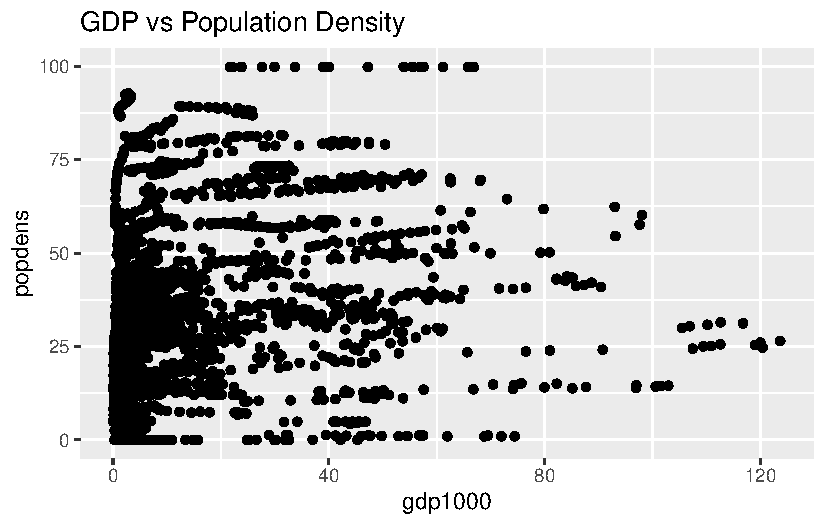
\includegraphics{week4_eda_inclass_files/figure-pdf/unnamed-chunk-7-1.pdf}

\begin{Shaded}
\begin{Highlighting}[]
\CommentTok{\#note missing values were removed}
\end{Highlighting}
\end{Shaded}

\begin{Shaded}
\begin{Highlighting}[]
\CommentTok{\#Bivariate analysis}

\CommentTok{\#temp vs. rainfall1000}
\FunctionTok{ggplot}\NormalTok{(finaldata, }\FunctionTok{aes}\NormalTok{(}\AttributeTok{x=}\NormalTok{temp, }\AttributeTok{y=}\NormalTok{rainfall1000)) }\SpecialCharTok{+} 
  \FunctionTok{geom\_point}\NormalTok{() }\SpecialCharTok{+} 
  \FunctionTok{labs}\NormalTok{(}\AttributeTok{title=}\StringTok{"Temperature vs Rainfall"}\NormalTok{)}
\end{Highlighting}
\end{Shaded}

\begin{verbatim}
Warning: Removed 20 rows containing missing values or values outside the scale range
(`geom_point()`).
\end{verbatim}

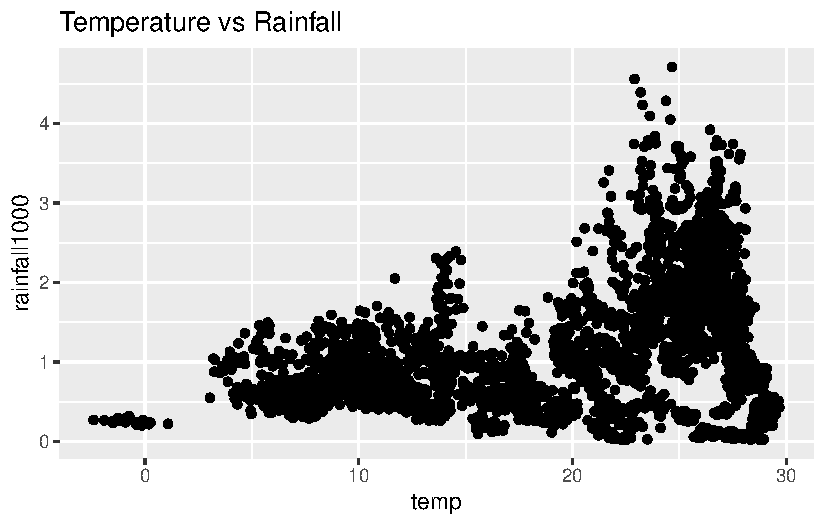
\includegraphics{week4_eda_inclass_files/figure-pdf/unnamed-chunk-8-1.pdf}

Lower temperature countries have less rainfall whereas for higher
temperature, it varies

\begin{Shaded}
\begin{Highlighting}[]
\CommentTok{\#Bivariate analysis}

\CommentTok{\#gdp1000 vs. Under5Mort}
\FunctionTok{ggplot}\NormalTok{(finaldata, }\FunctionTok{aes}\NormalTok{(}\AttributeTok{x=}\NormalTok{gdp1000, }\AttributeTok{y=}\NormalTok{Under5Mort)) }\SpecialCharTok{+} 
  \FunctionTok{geom\_point}\NormalTok{() }\SpecialCharTok{+} 
  \FunctionTok{labs}\NormalTok{(}\AttributeTok{title=}\StringTok{"GDP vs Under 5 mortality"}\NormalTok{)}
\end{Highlighting}
\end{Shaded}

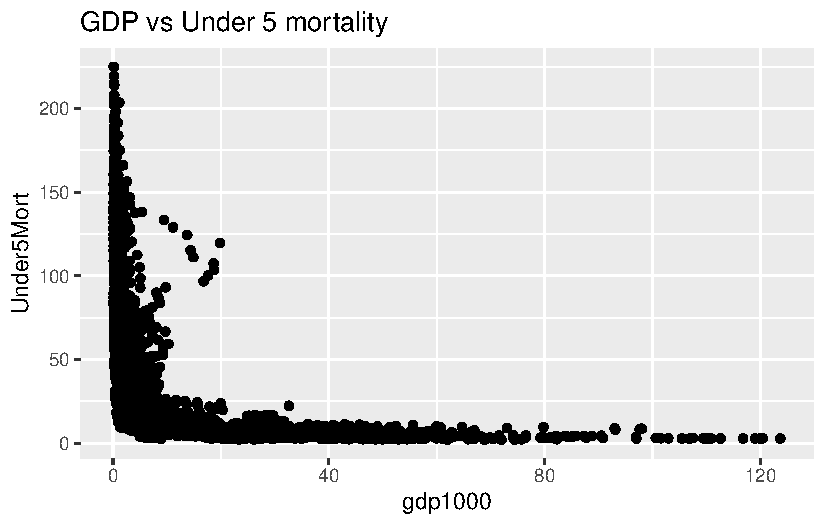
\includegraphics{week4_eda_inclass_files/figure-pdf/unnamed-chunk-9-1.pdf}

Countries with low GDP have substantially greater mortality rates for
children under 5.

\begin{Shaded}
\begin{Highlighting}[]
\CommentTok{\#Bivariate analysis}

\CommentTok{\#gdp1000 vs. NeonatalMort}
\FunctionTok{ggplot}\NormalTok{(finaldata, }\FunctionTok{aes}\NormalTok{(}\AttributeTok{x=}\NormalTok{gdp1000, }\AttributeTok{y=}\NormalTok{NeonatalMort)) }\SpecialCharTok{+} 
  \FunctionTok{geom\_point}\NormalTok{() }\SpecialCharTok{+} 
  \FunctionTok{labs}\NormalTok{(}\AttributeTok{title=}\StringTok{"GDP vs Neonatal Mortality"}\NormalTok{)}
\end{Highlighting}
\end{Shaded}

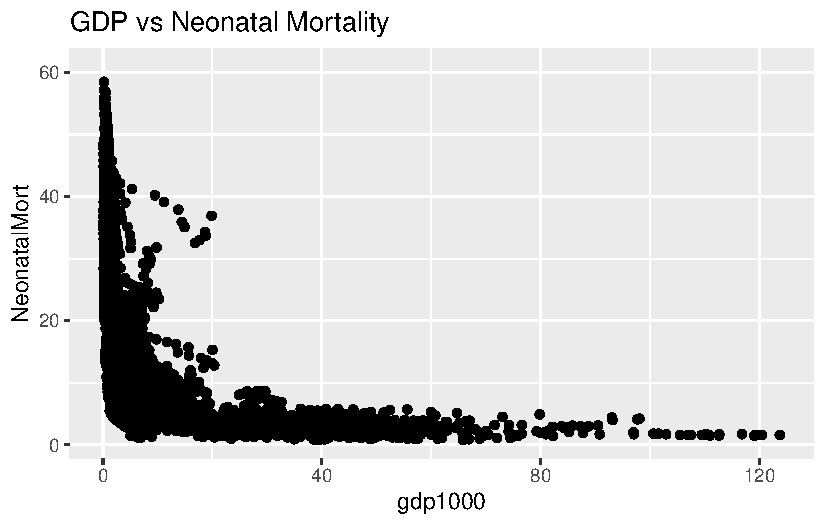
\includegraphics{week4_eda_inclass_files/figure-pdf/unnamed-chunk-10-1.pdf}

Countries with lower GDP have substantially higher neonatal mortality
rates

\begin{Shaded}
\begin{Highlighting}[]
\CommentTok{\#Bivariate analysis}

\CommentTok{\#gdp1000 vs. InfMort}
\FunctionTok{ggplot}\NormalTok{(finaldata, }\FunctionTok{aes}\NormalTok{(}\AttributeTok{x=}\NormalTok{gdp1000, }\AttributeTok{y=}\NormalTok{InfMort)) }\SpecialCharTok{+} 
  \FunctionTok{geom\_point}\NormalTok{() }\SpecialCharTok{+} 
  \FunctionTok{labs}\NormalTok{(}\AttributeTok{title=}\StringTok{"GDP vs Infant Mortality"}\NormalTok{)}
\end{Highlighting}
\end{Shaded}

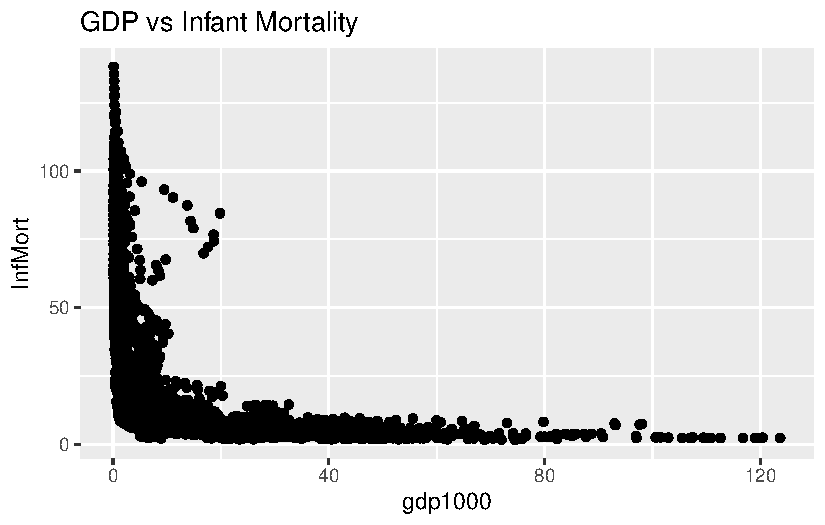
\includegraphics{week4_eda_inclass_files/figure-pdf/unnamed-chunk-11-1.pdf}

Countries with lower GDP have substantially higher infant mortality
rates




\end{document}
